
%
% Vorgehen : 
%           Darauf los schreiben
%           Ideen sammeln
%           Ordnen
%           Struktorieren
%           Einleitung
%           Überschrift suchen
%

\documentclass[bibtotoc,liststotoc,BCOR5mm,DIV12]{scrbook}
\usepackage{bibgerm}       % deutsche Literaturverzeichnisse
\usepackage[utf8]{inputenc}
\usepackage[ngerman]{babel}
\usepackage{graphicx} % Einfügen von Grafiken  - für PDF-Latex: .pdf und .png (.jpg möglich, sollte aber vermieden werden)
\usepackage{url}           % URL's (z.B. in Literatur) schöner formatieren
\usepackage[T1]{fontenc}
\usepackage{array}
\usepackage[none]{hyphenat}


%% Graphiken hier rein
\graphicspath{{./Bilder/}}

% ------------------------------------------------------------------------------
% \input{hyphenation} % in dieses File kommen Wörter die Latex nicht richtig trennt

%--------------------- globale includes 

% hyperref 
\usepackage{hyperref} % sorgt für für Hyperlinks in PDF-Dokumenten

\hypersetup{
    bookmarks=true,         % show bookmarks bar?
    unicode=false,          % non-Latin characters in Acrobat’s bookmarks
    pdftoolbar=true,        % show Acrobat’s toolbar?
    pdfmenubar=true,        % show Acrobat’s menu?
    pdffitwindow=false,     % window fit to page when opened
    pdfstartview={FitH},    % fits the width of the page to the window
    pdftitle={Projekarbeit Türschild},    % title
    pdfauthor={René Sodemann, Stefan Taute},     % author
    pdfsubject={Projektarbeit "Intelligentes Türschild"},   % subject of the document
    pdfcreator={René Sodemann, Stefan Taute},   % creator of the document
    pdfproducer={René Sodemann, Stefan Taute}, % producer of the document
    pdfkeywords={Android} {Türschild} {intelligent} {idc} {doorplate} {Samba} {Odys} {Xelio}, % list of keywords
    pdfnewwindow=true,      % links in new window
    colorlinks=true,       % false: boxed links; true: colored links
    linkcolor=blue,          % color of internal links
    citecolor=green,        % color of links to bibliography
    filecolor=magenta,      % color of file links
    urlcolor=cyan,           % color of external links
    linktocpage
}



% globale glossardatei 

% glossar package initialisierung 
\usepackage[
nonumberlist, %keine Seitenzahlen anzeigen
acronym,      %ein Abkürzungsverzeichnis erstellen
toc,          %Einträge im Inhaltsverzeichnis
section]      %im Inhaltsverzeichnis auf section-Ebene erscheinen
{glossaries}

% entfernt den punkt nach der glossar beschreibung
\renewcommand*{\glspostdescription}{}

\newglossary[slg]{symbolslist}{syi}{syg}{Symbolverzeichnis}

\makeglossaries

%% NOTE: wenn die einträge nicht referenziert werden gibt es auch keinen eintrag im glossar

\newglossaryentry{symb:Pi}{
    name=$\pi$,
    description={Die Kreiszahl.},
    sort=symbolpi, type=symbolslist
}
\newacronym{MS}{MS}{Microsoft}

%\newglossaryentry{symb:Pi}{
%name=$\pi$,
%description={Die Kreiszahl.},
%sort=symbolpi, type=symbolslist
%}
% oder 

% \newacronym{MS}{MS}{Microsoft}
% \newacronym{AD}{AD}{Active Directory\protect\glsadd{glos:AD}}
% \gls{AD}




\makeatletter
\def\thickhrulefill{\leavevmode \leaders \hrule height 1pt\hfill \kern \z@}
\renewcommand{\maketitle}{\begin{titlepage}%
    \let\footnotesize\small
    \let\footnoterule\relax
    \parindent \z@
    \reset@font
    \null
    \vskip 50\p@
    \begin{center}
      \hrule
      \vskip 1pt 
      \hrule
      \vskip 1pt
      {\huge \bfseries \strut \@title \strut}\par
      \vskip 1pt
      \hrule
      \vskip 1pt
      \hrule
    \end{center}
    \vskip 50\p@
    \begin{flushright}
      \Large \@author \par
    \end{flushright}
    \vfil
    \null
  \end{titlepage}%
  \setcounter{footnote}{0}%
}
\makeatother
\author{Isidore Ducasse, Comte de Lautréamont}
\author{Lautréamont}
\title{Les Chants de Maldoror}
\date{1874}

\makeatletter
\def\section{\@ifstar\unnumberedsection\numberedsection}
\def\numberedsection{\@ifnextchar[%]
  \numberedsectionwithtwoarguments\numberedsectionwithoneargument}
\def\unnumberedsection{\@ifnextchar[%]
  \unnumberedsectionwithtwoarguments\unnumberedsectionwithoneargument}
\def\numberedsectionwithoneargument#1{\numberedsectionwithtwoarguments[#1]{#1}}
\def\unnumberedsectionwithoneargument#1{\unnumberedsectionwithtwoarguments[#1]{#1}}
\def\numberedsectionwithtwoarguments[#1]#2{%
  \ifhmode\par\fi
  \removelastskip
  \vskip 3ex\goodbreak
  \refstepcounter{section}%
  \begingroup
  \noindent
  \leavevmode\Large\bfseries\raggedright
  \thesection\ #2\par\nobreak
  \endgroup
  \noindent\hrulefill\nobreak
  \vskip 2ex\nobreak
  \addcontentsline{toc}{section}{%
    \protect\numberline{\thesection}%
    #1}%
  }
\def\unnumberedsectionwithtwoarguments[#1]#2{%
  \ifhmode\par\fi
  \removelastskip
  \vskip 3ex\goodbreak
%  \refstepcounter{section}%
  \begingroup
  \noindent
  \leavevmode\Large\bfseries\raggedright
%  \thesection\ 
  #2\par\nobreak
  \endgroup
  \noindent\hrulefill\nobreak
  \vskip 2ex\nobreak
  \addcontentsline{toc}{section}{%
%    \protect\numberline{\thesection}%
    #1}%
  }

\makeatletter
\def\thickhrulefill{\leavevmode \leaders \hrule height 1ex \hfill \kern \z@}
\def\@makechapterhead#1{%
  \vspace*{10\p@}%
  {\parindent \z@ 
    {\raggedleft \reset@font
      \scshape \@chapapp{} \thechapter\par\nobreak}%
    \par\nobreak
    \vspace*{30\p@}
    \interlinepenalty\@M
    {\raggedright \Huge \bfseries #1}%
    \par\nobreak
    \hrulefill
    \par\nobreak
    \vskip 100\p@
  }}
\def\@makeschapterhead#1{%
  \vspace*{10\p@}%
  {\parindent \z@ 
    {\raggedleft \reset@font
      \scshape \vphantom{\@chapapp{} \thechapter}\par\nobreak}%
    \par\nobreak
    \vspace*{30\p@}
    \interlinepenalty\@M
    {\raggedright \Huge \bfseries #1}%
    \par\nobreak
    \hrulefill
    \par\nobreak
    \vskip 100\p@
  }}

\usepackage{amssymb,amsmath}
\usepackage{graphicx}
\usepackage{color}
\usepackage{listings}
\usepackage{courier}
\definecolor{darkgreen}{rgb}{0.0,0.6,0.0}
\lstset{
         basicstyle=\footnotesize\ttfamily, % Standardschrift
         numbers=left,               % Ort der Zeilennummern
         numberstyle=\tiny,          % Stil der Zeilennummern
         %stepnumber=2,               % Abstand zwischen den Zeilennummern
         numbersep=5pt,              % Abstand der Nummern zum Text
         tabsize=2,                  % Groesse von Tabs
         extendedchars=true,         %
         breaklines=true,            % Zeilen werden Umgebrochen
         keywordstyle=\color{darkgreen},
         frame=b,         
 %        keywordstyle=[1]\textbf,    % Stil der Keywords
 %        keywordstyle=[2]\textbf,    %
 %        keywordstyle=[3]\textbf,    %
 %        keywordstyle=[4]\textbf,   \sqrt{\sqrt{}} %
         stringstyle=\color{red}\ttfamily, % Farbe der String
         showspaces=false,           % Leerzeichen anzeigen ?
         showtabs=false,             % Tabs anzeigen ?
         xleftmargin=17pt,
         framexleftmargin=17pt,
         framexrightmargin=5pt,
         framexbottommargin=4pt,
         %backgroundcolor=\color{lightgray},
         showstringspaces=false      % Leerzeichen in Strings anzeigen ?        
 }
 \lstloadlanguages{% Check Dokumentation for further languages ...
         %[Visual]Basic
         %Pascal
         %C
         %C++
         %XML
         %HTML
         Java,
         bash
 }
%\captionsetup[lstlisting]{singlelinecheck=false, labelfont={blue}, textfont={blue}}
\usepackage{caption}
\DeclareCaptionFont{blue}{\color{blue}} 
\DeclareCaptionFont{white}{\color{white}}
\DeclareCaptionFormat{listing}{\colorbox[cmyk]{0.43, 0.35, 0.35,0.01}{\parbox{\textwidth}{\hspace{15pt}#1#2#3}}}
\captionsetup[lstlisting]{format=listing,labelfont=white,textfont=white, singlelinecheck=false, margin=0pt, font={bf,footnotesize}}




%--------------------- lokale includes 

%\newglossaryentry{symb:<symbolname>}{
%    name=$<command oder zeichen>$,
%    description=<beschreibung>,
%    sort=symbolpi, type=symbolslist
%}

%\newacronym{MS}{MS}{Microsoft}



\title{Projektarbeit}
\author{René Sodemann und Stefan Taute}
\date{today\setcounter{page}{0}\clearpage}

% --------------------------------------------------------------- BEGIN
\begin{document}

\raggedright
\frontmatter % Titelblätter und Erklärung jeweils spezifisch für die jeweilige Uni einbinden
    \begin{figure}[htb]
  \centering
  
\includegraphics[width=.4\textwidth]{ETI_logo.jpg}\\ % PNG-File
\end{figure}

  \centering
Projektarbeit
\vspace{\baselineskip}
im Studiengang Informatik

Fachbereich Elektrotechnik und Informatik 

\vspace{\baselineskip}
Thema: ``Intelligentes Türschild''
%% hier themanamen


\begin{center}
vorgelegt von

\vspace{\baselineskip}

Name: Sodemann \quad Vorname: René

Name: Taute \quad Vorname: Stefan

\vspace{\baselineskip}

Gutachter: Prof. Dr. rer. nat. Christian Bunse

\end{center}
    \tableofcontents 
    % Hier schreiben wir wer was gemacht hat

\chapter*{Aufgabenverteilung}

\begin{center}
\begin{tabular}[t]{|>{\centering\arraybackslash}p{.5\textwidth}|>{\centering\arraybackslash}p{.2\textwidth}|>{\centering\arraybackslash}p{.2\textwidth}|}
\hline
Aufgabe & René Sodemann & Stefan Taute\\
\hline
Versuche einen Digitalen Bilderrahmen als Intelligentes Türschild zu verwenden & X & X\\
\hline
Erstellung der Software für die Verwaltung am PC und der dazugehörigen Skripte & Software + BATCH-Skripte & BASH-Skripte\\
\hline
Erstellung einer APP für die Verwaltung auf dem Tablet &  & X\\
\hline
Recherche nach brauchbaren unterstützenden APP's & X & X\\
\hline
Konzept für die Netzwerkeinbindung des Türschilds &  & Konzept + Samba-VM\\
\hline
Erstellung der schriftlichen Ausarbeitung & X & X\\
\hline
\end{tabular}
\end{center}


    \chapter*{Zusammenfassung}
%Die deutsche Zusammenfassung. Halbe Seite.

% An der Universität Greifswald werden zur Unterstützung der Lehrenden und Lernenden ``\acs{Moodle}'' 
% und “\acs{LSF}” eingesetzt. Bei \acs{Moodle} handelt es sich dabei um ein \ac{Course-Management-System}, 
% welches kooperative Lehr- und Lernmethoden bereitstellt. Mit der
% Hilfe dieses Systems werden online Kursräume bereitgestellt, in denen Arbeitsmaterialien 
% und Lernaktivitäten veröffentlicht werden.
% Neben diesem System existiert an der Universität Greifswald ein Modul des Hochschul-Informationssystems 
% “\acs{HIS}” mit dem Namen “\acs{LSF}”, welches zur Repräsentation von
% Lehrveranstaltungen und allen dazu benötigten Ressourcen (wie z.B. Räume, Personen
% oder Lehrmittel) genutzt wird.
% Es soll nun im Rahmen einer Bachelorarbeit eine Schnittstelle zwischen beiden Systemen 
% erstellt werden, welche eine Kommunikation zwischen diesen ermöglicht. Es soll
% damit erreicht werden, dass die in \acs{HIS}-\acs{LSF} enthaltenen Daten auch innerhalb von \acs{Moodle}
% nutzbar sind, ohne die Inhalte per Hand zu übertragen und damit den Aufwand für Aktualisierungen zu verringern. 

Innerhalb der Gebäude der Fachhochschule Stralsund werden vor den Räumen Türschilder, Schaukästen oder Pinnwände genutzt, um allgemeine und raumspezifische Ankündigungen, mit Hilfe von Aushängen, zu verteilen. Damit ist ein einfacher Austausch von Informationen zwischen den Institutionen der Fachhochschule und deren Angehörigen möglich. 
Im Rahmen einer Projektarbeit soll nun eine Möglichkeit geschaffen werden, diese Aushänge in eine elektronische Form zu bringen, um so zum einen den Verwaltungsaufwand zu verringern und eine Möglichkeit zu schaffen Informationen effektiver zu verteilen.  

\mainmatter % die eigentliche Arbeit

%% TODO der von der Fh vorgegebene aufbau ist 
%% aufgabensstellung Thema
%% gliederung der aufgabe mit angaber der Seitenzahl
%% Textteil
%% zusammenfassung der einzelergebnisse
%% zusammenfassung aller formelzeichen 
%% Literaturverzeichniss

    
% Diesen Part des Dokuments als letztes schreiben


\chapter{ Einleitung }\label{chap:Einleitung}
\vspace{-3cm}
\begin{flushleft}
% 
% Die Einleitung schreibt man zuletzt, wenn die Arbeit im Großen und Ganzen schon fertig ist.
% (Wenn man mit der Einleitung beginnt - ein häufiger Fehler - braucht man viel länger und wirft sie später doch wieder weg). 
% Sie hat als wesentliche Aufgabe, den Kontext für die unterschiedlichen Klassen von Lesern herzustellen. Man muß hier die Leser für sich gewinnen. 
% Das Problem, mit dem sich die Arbeit befasst, sollte am Ende wenigsten in Grundzügen klar sein und dem Leser interessant erscheinen. 
% Das Kapitel schließt mit einer Übersicht über den Rest der Arbeit. Meist braucht man mindestens 4 Seiten dafür, mehr als 10 Seiten liest keiner.
% 
% Diese fragen Sollten beantwortet werden:
% Welche Fragestellung will ich behandeln ?
% Warum ist sie wichtig ?
% Warum ist sie nicht trivial ? ( bereits gelöst oder einfach lösbar )
% was möchte ich neues zur Lösung der Fragestellung beitragen ?
% Welche empirische Behandlung wähle ich zur Lösung der Fragestellung ?

\section{Motivation}
\label{sec:Motivation}
Im Rahmen einer Projektarbeit an der Fachhochschule Stralsund soll eine Methode entwickelt werden, um die innerhalb der Fachhochschulgebäude 
an den Türen angebrachten Schildern durch eine elektrische Lösung zu ersetzen. Dabei besteht die Hauptaufgabe darin den Schildern einen größeren Funktionsumfang zu geben und die dafür notwendige Anzahl an Arbeitsschritten so gering wie mögliche zu halten.  

\section{Bedeutung der Arbeit}
\label{sec:Bedeutung der Arbeit}
Die bisher an den Türen angebrachten Schildern werden hauptsächlich dafür genutzt um die Belegungspläne des jeweiligen Raumes oder um wichtige Informationen von Professoren zu veröffentlichen. Dabei ist darauf zu achten, dass nur ein begrenzt nutzbarer Raum für Informationen bereitsteht. Dadurch kommt es oft dazu, dass keine neuen Bekanntmachungen an den Schildern angebracht werden können und diese so verloren gehen, da sie nur in einem eingeschränkten Zeitraum aktuell sind. Dieser Mangel im Informationsfluss kann somit auch dazu führen, dass den Studenten Möglichkeiten entgehen, die ihre Studienzeit oder auch die erste Zeit im Berufsleben beeinflussen könnten. Beispiele dafür währen die Mitteilungen von Studien- oder Abschlussarbeiten an der Fachhochschule selbst oder in der freien Wirtschaft. 
Als nächster Punkt kann die Betreuung mehrerer Räume aufgeführt werden. Es muss in der derzeitigen Situation jeder Raum einzeln betreut werden, was eine vermehrte Zahl von Arbeitsschritten verlangt. Wird allerdings eine zentrale Lösung zur Verwaltung geschaffen, kann so die Zahl der nötigen Verwaltungsvorgänge verringert werden. 

\section{Zielsetzung}
\label{sec:Zielsetzung}
Mit dieser Arbeit soll eine Möglichkeit geschaffen werden, um die oben genannten Missstände zu beheben. Diese besteht darin die derzeitigen Türschilder durch eine elektrische Alternative zu ersetzen. Diese muss daraufhin so konfiguriert werden, dass sie eine Möglichkeit bietet zentral verwaltet zu werden und muss jedoch gleichzeitig gegen unbefugte Eingaben von Dritten geschützt werden. 

\end{flushleft}

    \chapter{ Grundlagen }\label{chap:Grundlagen}
\vspace*{-3cm}
\begin{flushleft}

In diesem Abschnitt der Arbeit, werden verschiedene Begriffe genauer erläutert, die benötigt werden, um die später beschrieben Bearbeitung
des Themas nachvollziehen zu können. Dazu gehören zum einen die Definitionen der eingesetzten Geräte und die dazugehörige Software.

\section{Digitaler Bilderrahmen}
Ausgangspunkt der Arbeiten am ``intelligenten Türschild'' war ein sogenannter digitaler Bilderrahmen der Firma Kodak. Da jedoch diese digitalen Bilderrahmen oft verschiedene Ausstattungen besitzen und sich somit gravierend unterscheiden können, wird zunächst eine Definition benötigt.

Bei einem digitalen Bilderrahmen handelt es sich um ein elektronisches Gerät, welches als Haupteinsatzgebiet die Wiedergabe von Bildmaterial hat. Es können dann noch je nach Modell weitere Funktionen (z.B. die Wiedergabe von Ton- und Videomaterial) und Ausstattungsmerkmale (z.B. Lautsprecher oder Kartenlesegeräte) vorhanden sein. Jedoch handelt es sich bei diesen Geräten nur um eine meist vereinfachte Form der derzeitigen Bildschirmtechnologie (z.B. LCD-Bildschirme, welche die Anzeige mit Hilfe von Flüssigkristallen erzeugen), welche dann mit einem Rahmen aus Kunststoff oder Metall ausgestattet werden.

Neben den unterschiedlichen Hardwareausstattungen verwenden die Hersteller verschiedene Softwarelösungen, um den Nutzer die Möglichkeit zu geben dem Bilderrahmen neues Bildmaterial zur Verfügung zu stellen oder um Bilder mit anderen Personen zu teilen. Die eingesetzte Software unterscheidet sich jedoch von Hersteller zu Hersteller. So setzt zum Beispiel Kodak als Software ``Kodak Pulse'' ein. Diese wird nun im nächsten Absatz genauer dargestellt, da sie für die weitere Bearbeitung des Themas nötig ist.

\section{Kodak Pulse}
Bei der Software die auf den Namen ``Kodak Pulse'' hört, handelt es sich um einen Service den die Firma Kodak ihren Kunden zur Verfügung stellt, um von Kodak produzierte digitale Bilderrahmen zu verwalten. Dazu muss jedoch der Bilderrahmen mit einem eingebauten W-Lan-Modul ausgerüstet sein. Der Nutzer muss nun wie in der Gebrauchsanweisung beschrieben den Bilderrahmen mit dem Internet verbinden. Im nächsten Schritt muss eine Anmeldung auf der Internetpräsenz von Kodak vorgenommen werden. Im Verlaufe dieser Anmeldung wird auch der Bilderrahmen mit dem Online-Konto verknüpft. Es besteht nun die Möglichkeit über die Weboberfläche Bilder zum Speicher des Rahmens hinzuzufügen oder zu löschen. Weiterhin kann der Nutzer die im Bilderrahmen vorhandenen Bilder mit Hilfe verschiedener Internetdienste wie Facebook oder Twitter mit anderen Personen teilen.

Jedoch ist die Fortführung dieses Dienstes gefährdet. Da in jüngster Vergangenheit immer mehr finanzielle Probleme bei Kodak auftraten, ist es nun schon zum Verkauf einiger Technologien und Diensten gekommen. Auch der ``Kodak Pulse''-Dienst steht zum Verkauf. Jedoch ist noch nicht sicher ob der Dienst im Falle eines Verkaufs noch weitergeführt wird. Dieser Fakt muss in diesem Abschnitt erwähnt werden, da dies den Verlauf der Bearbeitung entscheidend beeinflusst hat. 

\section{Android}
Bei dem Softwareprodukt ``Android'' handelt es sich um ein Betriebssystem, welches vorrangig auf mobilen Geräten wie Handys bzw. Smartphones und Tablets zum Einsatz kommt. Entwickelt wird diese Software von der ``Open Handset Alliance''. Dies ist ein Zusammenschluss mehrerer Unternehmen, welche das Ziel haben offene Standards für mobile Geräte zu schaffen. Bekannte Unternehmen die diesem Verbund angehören sind Google, Ebay, Vodafone und Gerätehersteller wie HTC, LG Electronics oder Samsung Electronics. 
Als Grundlage für das Android-Betriebssystem ist der Linux-Kernel (die unterste Softwareschicht eines Betriebssystems) in der Version 2.6 herangezogen worden. Seit Android-Version 4 ist auch ein Linux-Kernel der Version 3.x möglich. 
Das Endgerät, auf dem das Android-Betriebssystem arbeitet, kann mit Hilfe sogenannter ``Apps'' (Software die auf einem Android-Gerät nachträglich installiert werden kann) welche von verschiedenen Anbietern heruntergeladen werden können,um weitere Funktionen erweitert werden. Derzeit gibt es etwas mehr als 500.000 dieser Apps (Stand August 2012). Somit kann ein Endgerät je nach eingesetzten Programmen verschiedene Aufgaben erfüllen. 

\section{ADB}
Im späteren Verlauf der Projektarbeit kommt die sogenannte ``ADB'' zum Einsatz. Diese Abkürzung steht für ``Android Debug Bridge''. Hinter diesem Begriff verbirgt sich ein Tool, welches die direkte Kommunikation mit dem Gerät ermöglicht. Es wird ausschließlich über die Kommandozeile des PCs bedient und stellt verschiedene Befehle zur Verfügung. So können zum Beispiel Dateien vom PC auf das Handy kopiert werden oder auch vom Handy gelesen werden. Weiterhin besteht auch die Möglichkeit weitere Programme mit Hilfe dieses Tools auf dem Endgerät zu installieren. Damit bietet die Android Debug Bridge die Möglichkeit, am Gerät schwer zu findende Einstellungen vom PC vorzunehmen und diese Vorgänge zu vereinfachen. 

\section{Rooten von Android} 
Unter dem Begriff ``Root'' kann man den Administrator eines Gerätes oder eines Systems verstehen. Dieser ist dabei mit den größtmöglichen Rechten innerhalb des Systems ausgestattet. Standardmäßig besteht bei Android eine Einschränkung der Rechte. Somit muss ein sogenanntes ``Rooting'' durchgeführt werden, um diese Einschränkung zu umgehen. Die Prozedur für das Rooting unterscheidet sich von Gerät zu Gerät. Hat man allerdings nun vollen Zugriff auf das Gerät können nun Einstellungen durchgeführt werden, die vorher nicht möglich waren, zum Beispiel das Installieren eines veränderten Android-Betriebssystems (sogenannte ``Custom-Roms'') oder das nutzen von Apps die tief in das System eingreifen.

\section{Samba}
Des weiteren wird später in der Projektarbeit ein Netzwerkprotokoll namens ``SMB'' verwendet. Dieses Protokoll, wurde eigentlich für Netzwerkfreigaben unter Windows entwickelt. Die freie Software ``Samba'' macht es nun möglich unter Unix-Systemen ebenfalls das SMB-Protokoll zu verwenden. Diese Software wird in der Projektarbeit auch genau dazu verwendet. Sie soll später relativ kostengünstig die Inhalte der Türschilder vorhalten.
\end{flushleft}

% Hier werden zwei wesentliche Aufgaben erledigt:
% 
% Der Leser muß alles beigebracht bekommen, was er zum Verständnis der späteren Kapitel braucht. Insbesondere sind in unserem Fach die Systemvoraussetzungen zu klären, die man später benutzt. Zulässig ist auch, daß man hier auf Tutorials oder Ähnliches verweist, die hier auf dem Netz zugänglich sind.
% Es muß klar werden, was anderswo zu diesem Problem gearbeitet wird. Insbesondere sollen natürlich die Lücken der anderen klar werden. Warum ist die eigene Arbeit, der eigene Ansatz wichtig, um hier den Stand der Technik weiterzubringen? Dieses Kapitel wird von vielen Lesern übergangen (nicht aber vom Gutachter ;-), auch später bei Veröffentlichungen ist "Related Work" eine wichtige Sache.
% Viele Leser stellen dann später fest, daß sie einige der Grundlagen doch brauchen und blättern zurück. Deshalb ist es gut, Rückwärtsverweise in späteren Kapiteln zu haben, und zwar so, daß man die Abschnitte, auf die verwiesen wird, auch für sich lesen kann. Diese Kapitel kann relativ lang werden, je größer der Kontext der Arbeit, desto länger. Es lohnt sich auch! Den Text kann man unter Umständen wiederverwenden, indem man ihn als "Tutorial" zu einem Gebiet auch dem Netz zugänglich macht.
% 
% Dadurch gewinnt man manchmal wertvolle Hinweise von Kollegen. Dieses Kapitel wird in der Regel zuerst geschrieben und ist das Einfachste (oder das Schwerste weil erste).


    % Wie wird aktuell mit Türschildern gearbeitet
\chapter{ Stand }\label{chap:Stand}
\vspace{-3cm}
\begin{flushleft}
Dieses Kapitel setzt sich damit auseinander, wie aktuell die herkömmlichen Türschilder eingesetzt werden und welche möglichen Lösungen existieren, um diese zu ersetzen.

\section{Nutzung der Türschilder innerhalb der Gebäude der Fachhochschule} 
Zum aktuellen Zeitpunkt werden vor den Seminarräumen und den Laboren Metallschilder und vereinzelt Schaukästen bzw. Pinnwände eingesetzt, um Informationen und Stundenpläne zu veröffentlichen. Dabei ist für jeden Raum eine separate Betreuung nötig. Dies bedeutet, dass für jede neue Information die vor dem Raum publiziert werden soll, ein neues Dokument erstellt werden und platziert werden muss. Da wie bereits beschrieben nur ein sehr eingeschränkter Raum zur Verfügung steht, muss ebenfalls entschieden werden, welche Informationen nicht mehr benötigt werden und ausgetauscht werden können. Somit ist für einen eigentlich einfachen Vorgang ein dafür großer Arbeitsaufwand nötig. Ein weiterer Nachteil der bisherigen Lösung ist, dass durch die dezentrale Verwaltung es dazu kommen kann, dass ein und dieselbe Information mehrfach ausgehängt wird. Es kann also dazu kommen, dass an einer Stelle die Information bereits nicht mehr als aktuell angesehen wird, während es an anderer Stelle immer noch für aktuell gehalten wird. Es muss somit eine Lösung geschaffen werden, die eine zentrale Verwaltung ermöglicht um damit den Arbeitsaufwand zu verringern und gleichzeitig die Aktualität von Informationen zu verbessern. 
Für dieses Problem gibt es einen Lösungsansätze, welcher im nächsten Abschnitt genauer betrachtet wird. 

\section{Welche Technik gibt es bereits?}
Um das Problem des vermehrten Arbeitsaufwands und der doppelten Informationen zu lösen, entwickelten verschiedene Firmen sogenannte digitale Türschilder. Dabei handelt es sich meistens um besonders energiesparende PCs, welche zusammen mit einem Display in einem Gehäuse verbaut werden. Diese PCs können dann entweder über eine LAN- bzw. WLAN-Schnittstelle mit Informationen gefüllt werden. Bei manchen Modellen werden zusätzlich Kartenlesegeräte (z.B. für SD-Karten) verbaut. Dann kann mit Hilfe einer meist mitgelieferten Software die Türschilder verwaltet Dokumente auf diese übertragen werden. 
Nachteil dieser Lösung ist jedoch, dass diese Türschilder ausschließlich für dieses einzigen Einsatzzweck konzipiert wurden. Es gibt also keine Möglichkeit die Geräte anderweitig einzusetzen. Daraus resultiert also ein hoher Anschaffungspreis für ein ``einfaches'' Türschild. 
Weitere Lösungen basieren auf sehr ähnlichen Prinzipien und unterscheiden sich oft nur in der Verwaltungssoftware und darin, welche Formate das Türschild wiedergeben kann. 
\end{flushleft}



    \chapter{ Entwurf }
\vspace{-3cm}
\begin{flushleft}
Dieses Kapitel beschäftigt sich damit, welche Ziele die Arbeit verfolgt und wie diese mit den Anforderungen an das Endprodukt zusammengebracht werden. Weiterhin werden verschiedene Konzepte aufgezeigt, welche als Möglichkeit zur Problemlösung zur Verfügung standen. Diese werden daraufhin mit den Zielen und Anforderungen verbunden und es wird begründet, welche Lösung gewählt wurde.

\section{Ziele der Arbeit}\label{sec:Ziele der Arbeit}
Wie bereits beschrieben, verfolgt dieses Projekt verschiedene Intentionen. Diese werden an dieser Stelle noch einmal kurz aufgegriffen, um ein besseres Verständnis der folgenden Abschnitte zu gewährleisten.
\newline

Die Zielstellungen des Projekts lauten wie folgt:
\begin{itemize}
  \item Schaffung einer Lösung die bisherigen Türschilder zu ersetzen
  \item Verminderung des Verwaltungsaufwandes zur Eingabe und Pflege der zu publizierenden Informationen
\end{itemize}

Es muss allerdings berücksichtigt werden, dass diese Ziele nicht ohne Einschränkungen verfolgt werden können, denn sie sind an Anforderungen gebunden. Diese wurden bereits im Abschnitt \ref{sec:Anforderungen} ``Anforderungsdefinition'' vorgestellt.

\section{Konzepte zur Problemlösung}
Die in den Abschnitten \ref{sec:Ziele der Arbeit} und \ref{sec:Anforderungen} beschrieben Punkte müssen nun miteinander in Verbindung gebracht werden und es müssen, unter Berücksichtigung dieser Aspekte, mögliche Konzepte ausgearbeitet werden.
Diese Ausarbeitung und deren Ergebnisse werden in den folgenden Passagen genauer vorgestellt. Dabei werden zuerst verschiedene Lösungsansätze präsentiert, die dann bewertet werden. Im Anschluss daran wird einer der Vorschläge als Lösungsansatz gewählt und im nächsten Kapitel genauer betrachtet.

\subsection{Grundidee}
Für die Umsetzung des Projekts ist das bereits vorhandene Grundkonzept des energiesparenden PCs welcher mit einem Bildschirm in ein Gehäuse verbaut ist, die beste Grundlage. Jedoch ist es nicht möglich, die bereits fertigen Lösungen einzusetzen, da diese sehr kostenintensiv und unflexibel sind. Somit muss eine Abwandlung dieses Konzeptes entwickelt werden, um es für die Fachhochschule Stralsund einsatzfähig zu machen. 

\subsection{Nutzung eines digitalen Bilderrahmens als Türschild} \label{subsec:nutzungBilderrahmen}
Die erste hier gezeigte Umsetzung ist es, die Grundidee mit Hilfe eines digitalen Bilderrahmens umzusetzen. Die Entscheidung dafür fiel unter anderem, weil zwei Geräte der Marke ``Kodak'' (Modell: W1030) bereits in der Fachhochschule vorhanden waren und es auch weitere Modelle gibt, die kostengünstig zu erhalten sind. Bei den zwei vorhandenen Bilderrahmen handelt es sich um Bilderrahmen mit der ``Pulse''-Funktion. 

Moderne digitale Bilderrahmen haben einen großen Funktionsumfang. Sie besitzen ,je nach Modell, neben der Fähigkeit der Darstellung von Bildern auch die Wiedergabe Videos und Audioaufnahmen. Um die Verwaltung der Geräte zu vereinfachen bauen die Hersteller eine WLAN-Schnittstelle in die Geräte ein. Somit bietet ein digitaler Bilderrahmen die Voraussetzungen, um auch als digitales Türschild eingesetzt zu werden. 

Wie in Kapitel \ref{sec:Anforderungen} ``Anforderungen'' beschrieben soll eine zentrale Möglichkeit geschaffen werden das Türschild zu verwalten. Da die bereitgestellten Bilderrahmen die in Kapitel \ref{chap:Grundlagen} ``Grundlagen'' erwähnte ``Pulse''-Funktion besitzen, bietet es sich an diese Funktion zur Umsetzung zu nutzen. Dafür muss jedoch erst einmal ein Konto bei Kodak angelegt werden. Dafür werden der vollständige Name und eine E-Mail-Adresse benötigt. Ist der Bilderrahmen mit einem WLAN-Netzwerk verbunden, kann nun im Kodak-Pulse-Service der Rahmen mit Hilfe einer Kennnummer (zu finden am Karton des Bilderrahmens oder bei der Ersteinrichtung der WLAN-Verbindung) das Gerät dem Konto hinzugefügt werden. Nun ist die Verwaltung über einen Webbrowser möglich. Es können nun nach belieben Fotos hinzugefügt und auch wieder gelöscht werden. Dies kann auch für mehrere Rahmen getan werden. Dafür müssen diese dem ``Pulse''-Konto einfach hinzugefügt werden. 
Jedoch ist diese Kombination von Hardware und Software nicht die erhoffte Lösung. Es besteht das Problem, dass mit der Nutzung des ``Kodak-Pulse''-Service die auf den Bilderrahmen gespeicherten Daten auf einen Kodak-Server übertragen werden. Es werden also somit Informationen die nur für die Fachhochschule und dessen Angehörige bestimmt sind, nach Außen getragen. Ein weiterer Kritikpunkt ist die Abhängigkeit von einer externen Firma. Sollten Fehler oder Softwareausfälle auftreten, können diese nicht in eigener Verantwortung behoben werden und es kann damit nicht mehr die volle Funktionalität der Türschilder gewährleistet werden. Weiterhin muss in die Überlegungen mit einbezogen werden, dass die Firma ``Kodak'' aktuelle in einer wirtschaftlichen Krise steckt. Nach der Bekanntgabe der Insolvenz von Kodak werden verschiedenste Patente und Services zum Kauf angeboten. Unter anderem auch der ``Pulse''-Service. Es muss also damit gerechnet werden, dass der ``Pulse''-Service aus Kostengründen eingestellt wird oder an eine andere Firma verkauft wird. Wird der Service dann eingestellt, wird der Bilderrahmen nicht mehr als Türschild nutzbar sein. 
Es wird also eine andere Lösung benötigt. Diese sollte vor allem die Option bieten alle nötigen Komponenten innerhalb der Fachhochschule zu halten.  

Um diese Forderung zu erfüllen, müssten vor allem die benötigten Server innerhalb der Fachhochschule stehen. Um dies zu ermöglichen, gibt es ein von Hajo Noerenberg geschriebenes PHP-Skript, welches als ``Kodak Pulse Emulator'' benannt ist. Grundidee dieses Emulators ist es alle Anfragen und Verbindungen der Bilderrahmen die eigentlich die Kodakserver erreichen sollen an dieses PHP-Skript umzuleiten. Dort werden dann Antwortpakete erstellt, die der Bilderrahmen so auffasst, dass dieser denkt er habe sich erfolgreich mit den Kodakservern verbunden. Mit dieser Technik besteht die Möglichkeit die Daten, die die Geräte halten, auf einem Server der Fachhochschule zu speichern. 
Jedoch stellt sich heraus, dass dieses Skript nicht mit den aktuellen Firmwareversionen der Bilderrahmen funktioniert. In den früheren Versionen wurde der Hostname des SSL-Zertifikates nicht überprüft. Jedoch wurde diese Prüfung mit den neuen Firmwareversionen eingeführt. Somit ist auch diese Methode nicht für die Problemlösung einsetzbar. 

Da jedoch der Kodak-Bilderrahmen keine weiteren Schnittstellen zur Verfügung stellt, kann dieser nicht für die Problemlösung genutzt werden. Es werden also andere Geräte mit weiteren Schnittstellen benötigt. Eine solche Schnittstelle wäre zum Beispiel eine ``Samba''-Schnittstelle. Es handelt dabei um ein Protokoll, welches in der Lage ist die Datei- und Druckdienste von Microsoft Windows zu emulieren. Mit diesem Protokoll können also Dateien auf einem Server freigegeben werden, die dann vom Bilderrahmen gelesen und auch wiedergegeben werden können. Die Suche nach Bilderrahmen die eine solche Möglichkeit bieten, ergab dass es einige Sony Modelle mit dieser Technik gibt. Jedoch sind diese sehr kostenintensiv in der Anschaffung. Außerdem muss wieder bedacht werden, dass die Rahmen ausschließlich für diesen Zweck genutzt werden können. 
So entstand die Idee nach einem anderen Gerät zu suchen, welches kostengünstiger ist und zudem noch einen größeren Funktionsumfang als die Bilderrahmen bietet. Die Wahl fiel daraufhin auf Android-Tablets kleinerer Hersteller. Diese sind schon für etwa 100 Euro zu finden und bieten bei der Entwicklung völlige Freiheit, da sie Eigenentwicklungen zulassen. 
Die Umsetzung mit Hilfe eines Tablets wird im nächsten Abschnitt genauer beschrieben. 

\subsection{Nutzung eines Android-Tablets als Türschild}
Wie breits im vorherigen Abschnitt erwähnt, muss eine Alternative gefunden werden, die weitere Schnittstellen zur Verfügung stellt. Das beste Preis-/Leistungsverhältnis dafür bietet ein Tablet-PC auf Android-Basis. Diese bieten die Möglichkeit bei entsprechender Hardware alle nötigen Änderungen vorzunehmen. Es stellt sich nun die Frage, welche Hardwarekomponenten in einem solchen Tablet verbaut sein müssen. Im speziellen Falle des Projektes ist es vollkommen ausreichend, wenn eine WLAN-Schnittstelle vorhanden ist. Alle weiteren nötigen Schritte können dann mit Hilfe von Software durchgeführt werden. 
Im nächsten Schritt muss nun entschieden werden, welche Funktionen das Tablet bereitstellen muss, um als Bilderrahmen eingesetzt werden zu können. Dafür muss jedoch festgelegt werden, welche Version des Android-Betriebssystems eingesetzt werden soll, denn diese ist entscheidend dafür, welche Software auf dem Gerät lauffähig ist und welche nicht und welches Tablet dann gewählt wird. Um eine die größtmögliche Aktualität der Software gewährleisten zu können, sollte das Tablet mindestens die Android-Version 4.0 unterstützen. Durch die Festlegung dieser Eigenschaft wird gleichzeitig die Anzahl der möglichen Geräte eingeschränkt. Somit muss das Tablet nun eine W-LAN-Schnittstelle bieten, mit Android 4.0 arbeiten und sollte in der Anschaffung um 100 Euro liegen. Nach einiger Recherche fiel die Entscheidung auf das ``Odys Xelio''. Dieses Android-Tablet erfüllt somit alle Voraussetzungen, um als Ersatz für den Bilderrahmen zu dienen. 
Nun müssen dem Tablet die nötigen Funktionen mit Hilfe von Software beigebracht werden. Es werden für den Einsatz folgende Funktionen benötigt:
\begin{itemize}
  \item das Tablet muss gegen unbefugte Eingaben von Dritten geschützt werden
  \item das Tablet muss in der Lage sein eine Fotopräsentation darzustellen
  \item das Tablet muss die Möglichkeit bieten, Bildmaterial von einer entfernten Quelle beziehen zu können
  \item das Tablet sollte so stromsparend wie möglich arbeiten
\end{itemize}

Diese Anforderungen müssen nun noch weiter präzisiert werden, denn nur so ist es möglich die richtigen Softwarekomponenten für den Produktiveinsatz auszuwählen. 
In Bezug auf den Punkt ``Verhindern von unbefugten Eingaben von Dritten'' bedeutet dies, dass jegliche Eingabemöglichkeit über das Touchdisplay verhindert werden muss, sobald eine Photopräsentation aktiviert ist. Da jedoch danach immer noch die Möglichkeit besteht mit Hilfe der Hardwaretasten des Odys Xelio zu navigieren, müssen diese ebenfalls deaktiviert werden. Somit ist gewährleistet, dass ein Außenstehender keine Mittel besitzt Einstellungen am Tablet zu verändern. 

Die Funktionalität der Darstellung einer Fotopräsentation ist deswegen notwendig, da die gezeigten Informationen als Bilddatei vorliegen. Somit muss das Tablet aus einer gegebenen Quelle die Dateien lesen und diese dann über den Bildschirm wiedergeben.

Die zuvor angesprochene Quelle besitzt dabei jedoch eine besondere Eigenschaft. Diese soll sich nämlich nicht direkt auf dem Tablet, sondern      
auf einem externen Medium befinden. Das Tablet selbst soll diese auslesen und dann, wenn es für die Ausführung nötig ist, zwischenspeichern und daraufhin wiedergeben.

Der letzte angesprochene Punkt ist der Energieverbrauch des Gerätes. Da die dargestellten Informationen nicht 24 Stunden pro Tag zugänglich sein müssen, soll eine Möglichkeit geschaffen werden, den Energieverbrauch in einem bestimmten Zeitrahmen zu senken. Ein Beispiel dafür wäre, dass der Bildschirm sich in den Stunden von 21 Uhr bis 7 Uhr ausschaltet oder dass das Gerät in diesen Stunden in einen energiesparenden Modus wechselt. 

All diese genannten Funktionen bietet das Odys Xelio jedoch nicht in seiner Standardkonfiguration. Es muss also noch mit Hilfe von weiteren Softwareprodukten diese Funktionalitäten geschaffen werden. Welche Software bzw. Techniken das im einzelnen ist, wird im nächsten Abschnitt genauer beschrieben. 
%danach anforderungen spezifizieren
%erklären, dass das tablet das so nicht kann
%hinweis darauf, dass im nächsten abschnitt darauf eingegangen wird
\end{flushleft}

% st das zentrale Kapitel der Arbeit. Hier werden das Ziel sowie die eigenen Ideen, Wertungen, Entwurfsentscheidungen vorgebracht. Es kann sich lohnen, verschiedene Möglichkeiten durchzuspielen und dann explizit zu begründen, warum man sich für eine bestimmte entschieden hat. Dieses Kapitel sollte - zumindest in Stichworten - schon bei den ersten Festlegungen eines Entwurfs skizziert und in Stichworten geschrieben werden. Es wird sich aber in einer normal verlaufenden Arbeit dauernd etwas daran ändern. Das Kapitel darf nicht zu detailliert werden, sonst langweilt sich der Leser. Es ist sehr wichtig, das richtige Abstraktionsniveau zu finden. Bei der Verfassung sollte man auf die Wiederverwendbarkeit des Textes achten.
% 
% Plant man eine Veröffentlichung aus der Arbeit zu machen, können von diesem Kapitel Teile genommen werden. Das Kapitel wird in der Regel wohl mindestens 8 Seiten haben, mehr als 20 können ein Hinweis darauf sein, daß das Abstraktionsniveau verfehlt wurde.


    \chapter{ Implementation }
Hier greift man einige wenige, interessante Gesichtspunkte der Implementierung heraus. Das Kapitel darf nicht mit Dokumentation oder gar Programmkommentaren verwechselt werden. Es kann vorkommen, dass sehr viele Gesichtspunkte aufgegriffen werden müssen, ist aber nicht sehr häufig. Zweck dieses Kapitels ist einerseits, glaubhaft zu machen, daß man es bei der Arbeit nicht mit einem "Papiertiger" sondern einem real existierenden System zu tun hat. Es ist sicherlich auch ein sehr wichtiger Text für jemanden, der die Arbeit später fortsetzt. Der dritte Gesichtspunkt dabei ist, einem Leser einen etwas tieferen Eindruck in die Technik zu geben, mit der man sich hier beschäftigt. Schöne Bespiele sind "War Stories", also Dinge mit denen man besonders zu kämpfen hatte, oder eine konkrete, beispielhafte Verfeinerung einer der in Kapitel 3 vorgestellten Ideen. Auch hier gilt, mehr als 20 Seiten liest keiner, aber das ist hierbei nicht so schlimm, weil man die Lektüre ja einfach abbrechen kann, ohne den Faden zu verlieren. Vollständige Quellprogramme haben in einer Arbeit nichts zu suchen, auch nicht im Anhang, sondern gehören auf Rechner, auf denen man sie sich ansehen kann.
% hier könnte drin stehen:
% Versuch mit dem PHP-Skript für Kodak-Pulse und Router (DNS-MASQ, SSL-Strip)
% Entwicklung der Anwendersoftware und Androidapp (welche Funktionen brauch die app, wie eingepflegt, energieprobleme?)
    \chapter{ Leistungsbewertung }\label{chap:Leistungsbewertung}
Zu jeder Arbeit in unserem Bereich gehört eine Leistungsbewertung. Aus diesem Kapitel sollte hervorgehen, welche Methoden angewandt worden, die Leistungsfähigkeit zu bewerten und welche Ergebnisse dabei erzielt wurden. Wichtig ist es, dem Leser nicht nur ein paar Zahlen hinzustellen, sondern auch eine Diskussion der Ergebnisse vorzunehmen. Sehr gut ist, wenn man zunächst diskutiert und plausibel macht, welche Ergebnisse man erwartet, und dann eventuelle Abweichungen diskutiert.

    \chapter{ Schlussfolgerung }
Dieses Kapitel ist sicherlich das am Schwierigsten zu schreibende. Es dient einer gerafften Zusammenfassung dessen, was man gelernt hat.Es ist möglicherweise gespickt von Rückwärtsverweisen in den Text, um dem faulen aber interessierten Leser (der Regelfall) doch noch einmal die Chance zu geben, sich etwas fundierter weiterzubilden. Manche guten Arbeiten werfen mehr Probleme auf als sie lösen. Dies darf man ruhig zugeben und diskutieren. Man kann gegebenenfalls auch schreiben, was man in dieser Sache noch zu tun gedenkt oder den Nachfolgern ein paar Tips geben. Aber man sollte nicht um jeden Preis Fragen, die gar nicht da sind, mit Gewalt aufbringen und dem Leser suggerieren, wie weitsichtig man doch ist. Dieses Kapitel muß kurz sein, damit es gelesen wird.
    
    \chapter{ Zusammenfassung }
\vspace{-3cm}
\begin{flushleft}
Im Rahmen dieser Projektarbeit wurde mit Hilfe von Java, dem Betriebssystem ``Android'' und dafür entwickelte Software eine Möglichkeit entwickelt, welche ein Tablet-PC in einen digitalen Bilderrahmen verwandelt, um so den Aufwand der Pflege von Informationen zu verringern.
\newline

Im Einleitungskapitel Kapitel \ref{chap:Einleitung} wurde ein Überblick darüber gegeben, wie die aktuelle Situation in Bezug auf die Verteilung von Informationen an der Fachhochschule Stralsund aussieht und welche Veränderungen an diesem Zustand vorgenommen werden sollen. 
\newline

Daran anschließend wurde im Kapitel \ref{chap:Grundlagen} ``Grundlagen'' aufgezeigt, welche Technologien in der Arbeit genutzt werden, um die gestellte Aufgabe zu lösen. 
\newline

In Kapitel \ref{chap:Stand} ``Stand'' wurde noch einmal genauer beschrieben, wie die Türschilder bzw. Schaukästen genutzt werden und es wurde die Problemstellung noch einmal genauer definiert. Ebenfalls wurde eine bereits vorhandene Lösung für das Problem präsentiert und warum dieses nicht genutzt werden kann. 
\newline

Der nächste Abschnitt (Kapitel \ref{sec:Anforderungen}) gab eine Übersicht darüber, unter welchen Anforderungspunkten die Entwicklung des Projekts vollzogen werden sollte. Es erfolgte dafür eine Einteilung in funktionale und nichtfunktionale
Anforderungen. Dabei stützte sich die Erstellung der funktionalen Anforderungen auf die Formulierung von User Stories und die nichtfunktionalen Anforderungen auf den Standard ``ISO 9126''.
\newline

Das Kapitel \ref{chap:Entwurf} ``Entwurf'' setzte sich damit auseinander, welche Umsetzungsmöglichkeiten es für das vorliegende Problem gibt. Dabei entstanden zwei verschiedene Ansätze.
Als erstes wurde dabei Untersucht, ob ein digitaler Bilderrahmen als Lösung einsetzbar ist. Jedoch wurde während der Bearbeitung festgestellt, dass auf Grund einer neuer Firmwareversion des Bilderrahmens dieser nicht mehr für die Umsetzung geeignet ist. 
Es musste nun eine neue Option gesucht werden, um das Projekt weiterzuführen. Dabei fiel die Wahl auf einen Tablet-PC auf Android-Basis. Das Kapitel beschrieb daraufhin die Vorzüge des Tablet-PCs gegenüber dem Bilderrahmen und welche Arbeiten noch am Tablet durchgeführt werden müssen.
\newline

\newpage
Im Abschnitt \ref{chap:Umsetzung} wurde nun genauer darauf eingegangen, wie die im vorherigen Kapitel beschriebenen nötigen Arbeitsschritte umgesetzt wurden und wie die Versuche mit den digitalen Bilderrahmen aussahen.
\newline

%Das Kapitel \ref{chap:Leistungsbewertung} zeigte, welche zuvor aufgezeigten Probleme gelöst werden konnten und an welchen Stellen noch Verbesserungen vorgenommen werden können.

Das Kapitel \ref{chap:Ausblick} zeigte,was noch zu einer komfortablen endgültigen Lösung in der Fachhochschule umgesetzt werden müsste.
\end{flushleft}

% Zu einer runden Arbeit gehört auch eine Zusammenfassung, die eigenständig einen kurzen Abriß der Arbeit gibt. Eine halbe bis ganze DINA4 Seite ist angemessen. Dafür läßt sich keine Gebrauchsanweisung geben (für irgendetwas müssen die Betreuer ja auch noch da sein). Jetzt sollen noch einige, eher generelle Hinweise gegeben werden:


    \chapter{Gebrauchsanweisung}
\vspace*{-3cm}
\begin{flushleft}
In diesem Kapitel werden die Funktionen erläutert, die die mitgelieferte Software bietet. Dabei erfolgt eine Unterteilung in die Erstellung von Notizen und die Wartung bzw. Inbetriebnahme des Xelio-Tablets. Weiterhin wird die für die Umsetzung des Projekts nötige Treiberinstallation erklärt. 

\section{Installieren des Treibers}
% TODO USB-Debugging aktivieren erwähnen

\section{Bedienung der Software am PC}
\subsection{Erstellung einer Notiz}
Um für das Tablet eine Nachricht zu erzeugen, muss die eigentliche Textnachricht in eine Bilddatei umgewandelt werden. Um diese Umwandlung zu vollziehen kann die mitgegebene Software genutzt werden. Dafür müssen folgende Schritte durchgeführt werden:
\begin{itemize}
  \item Klicken sie auf den Button ``Vorlage wählen''.
    \subitem Es öffnet sich nun ein Dialog für die Auswahl einer Bilddatei. Diese wird später der Hintergrund sein, auf dem sich die 			 Nachricht befindet. Bestätigen Sie ihre Auswahl mit ``öffnen''.
    \subitem Es wurde nun der Dateipfad zum Hintergrund in das entsprechende Textfeld eingetragen. 
    
  \item Im Feld ``Nachricht'' geben Sie nun die Nachricht ein, die auf dem Tablet erscheinen soll. 
    \subitem Hinweis: Es können bei der Eingabe selbstständig Zeilenumbrüche vorgenommen werden. Jedoch erfolgt seitens der Software noch 	  	 eine Kontrolle ob die eingegebene Nachricht für das Bild passend ist. Sollte dies nicht der Fall sein, werden weitere 	
	     Zeilenumbrüche eingefügt.  
	     
  \item Im nächsten Schritt kann nun mit Hilfe der Combobox die Schriftgröße der zu erscheinenden Nachricht eingestellt werden. 
  
  \item Sie können sich nun vor dem eigentlichen Erstellen der benötigten Bilddatei noch eine Vorschau der Notiz zeigen lassen. Dazu drücken   
        Sie auf den Button ``Vorschau anzeigen''. Es erscheint nun ein Fenster mit der Vorschau, welches Sie nach der Betrachtung wieder schließen können.
        
  \item Es können nun noch Veränderungen an der Nachricht vorgenommen werden. Entspricht die Notiz den Anforderungen kann mit einem Klick 	
	auf den Button ``Notiz erstellen'' ein Dialog zum Speichern der Bilddatei aufgerufen werden. Es muss nun ein Speicherort bestimmt werden und die Datei muss benannt werden. 
	
  \item Nun kann die Datei auf das Tablet übertragen werden und daraufhin auf dem Tablet angezeigt. 
\end{itemize}

Im nun folgenden Abschnitt wird der zweite Teil der Software genauer vorgestellt.

\subsection{Softwareinstallation und Wartung}
In diesem Absatz werden die Funktionen der vier verschiedenen Buttons im unteren Bereich der Software erklärt.

\begin{itemize}
  \item Button ``Xelio Rooten''
    \subitem Ist das Xelio an den PC angeschlossen und ist das USB-Debugging aktiviert, kann mit einem Klick auf den Button das Rooting des 	
	     Tablets starten. Während dieses Vorgangs kommt es zu einem Neustart des Geräts. Danach besitzt man Root-Zugang auf dem Xelio.
	     
  \item Button ``Software installieren''
    \subitem Nachdem das Tablet gerootet wurde, kann nun die Installation der nötigen Software erfolgen. Dies geschieht mit diesem Button. 	
	     Nach einem Klick erscheint ein Fenster welches den aktuellen Status ausgibt. Sollte sich das Fenster von alleine schließen, stoßen Sie den Vorgang erneut an. 
	 
  \item Buttons ``Hardwarebuttons aktivieren'' und ``Hardwarebuttons deaktivieren''
    \subitem Um das Tablet vor unerwünschten Eingaben zu schützen wurde die Möglichkeit geschaffen, die an der Vorderseite angebrachten 	
             Hardwarebuttons zu deaktivieren. Müssen nun allerdings doch Eingaben am Tablet selbst erfolgen, kann mit Hilfe der Software die Buttons wieder aktiviert werden. Für beide Fälle gilt, dass ein Neustart des Systems benötigt wird. Während der Ausführung des Befehls erscheint wieder ein Fenster, welches den aktuellen Status ausgibt. Sollte sich dieses wieder von alleine schließen, starten Sie den Vorgang bitte erneut.
\end{itemize}


\section{Bedienung der Verwaltungsapplikation auf dem Tablet}
  Nachdem das Tablet durch die entwickelte Verwaltungssoftware für den PC vorbereitet und außerdem ein entsprechender Samba-Server eingerichtet wurde, kann es nun auf dem Tablet weitergehen.
  \begin{itemize}
  \item{Konfigurieren des WLAN}
    Auf dem Tablet muss zunächst das WLAN konfiguriert werden.
    \begin{itemize}
      \item Klicken sie in der unteren rechte Ecke des Touchscreens auf die Uhr. Dort sollte sich ein Popup-Dialog öffnen.
      \item Dort klicken sie bitte auf das obere Feld mit der Uhr, daraufhin sollte sich der Dialog aktuallisieren.
      \item Hier kann man nun auf die Schaltfläche ``WLAN'' klicken, worauf sie in die WLAN-Einstellungen gelangen.
      \item Auf der rechten Seite sind nun die gefundenen WLAN-Netzwerke zusehen. Falls nicht, müssen sie auf der linken Seite den WLAN-Schalter auf ``AN'' stellen.
      \item Nachdem sie sich im WLAN mit vorhandenen Samba-Server angemeldet haben, können sie in der unteren linken Ecke auf die Zurück-Schaltfläche klicken.
    \end{itemize}
  \end{itemize}
  Die restlichen Einstellungen können nun über die entwickelte Verwaltungs-Applikation ``InteligentDoorplateControl'' vorgenommen werden.
  \subsection{Konfigurieren der Applikation - NoLock}
    Die NoLock-Applikation dient dazu, zu verhindern das das Tablet nach dem Bildschirm ausschalten den Lockscreen aktiviert.
    \begin{itemize}
      \item Starten sie die App mittels der Schaltfläche ``Configure NoLock!''.
      \item Falls dort noch ``Lock enabled'' steht klicken sie einmal dort drauf und schon sollte dort ``Lock disabled'' erscheinen, womit der Lockscreen abgeschaltet wurde.
      \item Falls dort schon ``Lock disabled'' zu sehen ist, ist der Lockscreen bereits deaktiviert. Das liegt daran das dies nur einmal gemacht werden muss, solange das Tablet nicht zurückgesetzt wird.
    \end{itemize}
  \subsection{Konfiguration der Applikation - ScreenOff}
    Die ScreenOff App ist ein wesentlicher Bestandteil des Standby-Service. Die Applikation wird automatisch ausgeführt wird, wenn die konfigurierte Sleeptime erreicht ist.
    Die Konfiguration von ScreenOff, ist eigentlich nur eine Aktivierung dieser. Die Applikation benötigt die freigabe als Geräteadministrator. Man muss hierbei die App nur zweimal starten und zwar über den Button ``Configure ScreenOff!''. Beim ersten mal werden einige Hinweise gegeben, diese kann man mit \textit{OK} bestätigen. Das zweite mal wird gefragt ob die Applikation Geräteadministrator werden darf, was man mit \textit{Aktivieren} bestätigen muss.
    Daraufhin ist die Applikation ordnungsgemäß aktiviert. Falls man die funktionalität prüfen will, kann  man einfach noch mal auf den entsprechenden Button drücken wodrauf das Tablet den Bildschirm ausschalten sollte. Solange die App nicht zurückgesetzt wird, bleibt die Aktivierung erhalten.
  \subsection{Konfigurieren der Applikation - PCFileSync}
  Die PCFileSync-Applikation dient dazu, ein bestimmtes Verzeichnis mit einer entsprechenden Netzwerkfreigabe, die in diesem Projekt über das SMB-Protokoll realisiert wird, zu synchronisieren.
    \begin{itemize}
      \item Starten sie die App mittels der Schaltfläche ``Start/configure PcFileSync!''.
      \item In der App rufen sie nun das Kontextmenü über die Hardware bzw. Software Options-Taste auf.
      \item Dort klicken sie nun auf ``Settings'' und im darauf folgenden Dialog ``Profiles settings''.
      \item Hier muss nun ein neues Profil angelegt werden, um die Synchronisation mit einem lokalen Verzeichnis und einem entsprechenden Netzwerkverzeichnis sicherzustellen. Dazu klicken sie lange in die freie Fläche der Activity, bis sich ein Dialog öffnet. Dort wählen sie ``Add SMB Profile''.
      \item Daraufhin gelangen sie zu einer Activity mit vielen Einstellungsmöglichkeiten. In der folgenden Abbildung ist zu sehen wie man diese Felder ausfüllen sollte, natürlich mit kleineren Anpassungen wie Raumnummer usw.
      \end{itemize}
      \begin{figure}[htb]
        \centering
        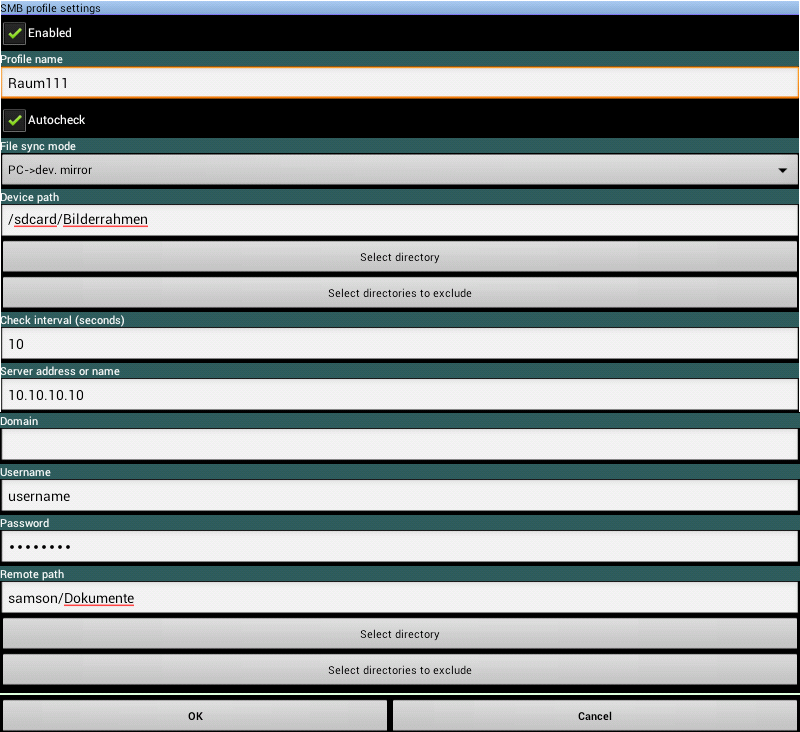
\includegraphics[width=.7\textwidth]{pcfilsync_conf.png}\\ % PNG-File
      \end{figure}
      Nun ist die App fertig konfiguriert und der Synchronisation-Service sollte schon automatisch gestartet sein.
      Ab dem zweiten Mal, muss die PcFileSync-App nur noch einmal gestartet werden, damit der Service startet, die Konfiguration bleibt erhalten.    
  \subsection{Konfigurieren der Applikation - PhotoFrameApp}
  	Die PhotoFrame-Applikation dient dazu, dass die Bilder aus dem synchronisierten Verzeichnis mittels einer Diashow ausgegeben werden.
    \begin{itemize}
      \item Starten sie die App mittels der Schaltfläche ``Start/configure PhotoFrameApp!''.
      \item Am oberen Rand sehen sie dann in der App eine Schaltfläche mit einem kleinen Zahnrad, klicken sie dort drauf, um in die Einstellungen zu gelangen.
      \item Angelangt im Einstellungs-Dialog, legt man zuerst das Intervall zwischen den Bildern fest. Zum Beispiel ein Intervall von 20 Sekunden.
      \item Als nächstes legt man die Art der Reihenfolge der Diashow fest. Im Fall eines Türschilds, würden wir die Reihenfolge nach Datum epmfehlen.
      \item Daraufhin muss das erneute einlesen des Ordners aktiviert werdenm, dazu machen sie bitte einen Haken bei ``Erneutes Laden einschalten''. Darunter legen sie das Intervall fest, wie oft der Ordner neu eingelesen wird. Wir würden ein Intervall von 30 Sekunden vorschlagen, das sollte ausreichend oft sein.
      \item Darauffolgend kann man eine Option aktivieren, die es veranlasst, dass nach dem ersten mal starten einer Diashow, die App bei nächsten Start wieder die Diashow im selben Ordner startet. Diese Option empfehlen wir ebenfalls, man aktiviert sie mit einem Haken bei Punkt ``Nach dem Neustart automatisch Fotos anzeigen.''.
      \item Nun folgen noch ein paar Anzeigeoptionen für die Diashow, diese sind natürlich nur eine Empfehlung. Sie beeinträchtigen also nicht die Funktion des Tablets als intelligentes Türschild.
      \begin{itemize}
        \item Als erstes kann man das Standardlayout zur Anzeige der Bilder auswählen. Wir würden hier das Layout ``Vollbild Fotos'' empfehlen
        \item Danach kommt der Punkt ``Deckkraft starten'', hier kann man einstellen, ob die Bilder nachdem erscheinen langsam heller werden. Diese Option ist nach unserer Meinung, bei einem Türschild nicht sehr sinnvoll, also würden wir empfehlen diesen auf dem Wert ``255'' zu belassen.
        \item Als nächstes kann man aktivieren bzw. deaktivieren ob in der Diashow eine Foto Nummerierung zusahen sein soll. Wir würde die Option deaktivieren, ist bei einem Türschild nicht relevant.
        \item Daraufhin kann man auswählen ob der Dateiname angezeigt werden soll, was wir ebenfalls nicht empfehlen würden.
        \item Zum Schluss kommen die beiden Optionen ``Zeige Vollbild'', die Bilder werden also möglichst groß skaliert in Abhängigkeit der Auflösung des Bildschirms und ``Werden im Querformat.'', also alle Bilder werden ins Querformat gebracht. Diese beiden Optionen würden wir aktivieren.
      \end{itemize}
    \end{itemize}
    Damit ist die Konfiguration der PhotoframeApp weitestgehend abgeschlossen, beim endgültigen starten der Applikation, nach der Einrichtung des Standby-Service, muss man dann nur noch den entsprechenden Ordner, der mittels PcFileSync synchronisiert ist, auswählen.
  \subsection{Standby-Service konfigurieren}
    Der Standby-Service wurde dazu entwickelt, das Tablet zu bestimmten Zeiten aus dem Standby aufzuwecken bzw. in den Standbymodus zu versetzen.
    \begin{itemize}
      \item In der rechten Spalte der IDC-App haben wir zwei TimePicker zum festlegen der Wake-UP- und Sleep-Time. Diese legt man nun nach seinen Wünschen fest.
      \item Danach können sie über den Button ``Start Standby \& NoTouch Service'' den Service starten.
      \item Vor dem Start wird auch in der Applikation noch mal der Hinweis gegeben, dass sie noch ca. 5 Minuten haben bis der Touchscreen gesperrt wird. Danach ist das Tablet nur noch durch einen Neustart wieder normal zu verwenden.
    \end{itemize}
    In der verbleibenden Zeitspanne, muss nun endgültig die PhotoFrameApp gestartet und die Diashow ausgeführt werden. Daraufhin ist das Tablet nun so konfiguriert, das es sich mit dem gewählten Verzeichnis synchronisiert, es eine Diashow mit dessen Inhalt ausgibt, es nicht von Unbefugten benutzt werden kann und es sich zu bestimmten Zeiten in den Standbymodus versetzt und daraus auch wieder erwacht.
\end{flushleft}


\backmatter % ab hier keine Nummerierung mehr
    \listoffigures
    \bibliographystyle{geralpha}
    %% TODO testen ob nicht am anfang besser is
    % glossar
    \printglossary[style=altlist,title=Glossar]
    % abkürzungen
    % TODO \deftranslation[to=German]{Acronyms}{Abkürzungsverzeichnis}
    \printglossary[type=\acronymtype,style=long]
    % symbole
    \printglossary[type=symbolslist,style=long]
    % TODO bib daten in ordner
    %\bibliography{./Bib/stud77}
    %\chapter{Selbstständigkeitserklärung}
Ich versichere, die von mir vorgelegte Arbeit selbständig verfasst zu haben. Alle
Stellen, die wörtlich oder sinngemäß aus veröffentlichten oder nicht veröffentlichten
Arbeiten anderer entnommen sind, habe ich als entnommen kenntlich gemacht.
Sämtliche Quellen und Hilfsmittel sind angegeben. Die Arbeit hat mit gleichem bzw.
in wesentlichen Teilen gleichem Inhalt noch keiner Prüfungsbehörde vorgelegen.

%\vfill
\vspace{2cm}

\begin{tabular}{lp{2em}l}
 \hspace{5cm}   && \hspace{4cm} \\\cline{1-1}\cline{3-3}
 Ort, Datum     && Unterschrift
\end{tabular} 
%\Unterschrift{Greifswald}{\today}{René Sodemann}

 

\end{document}

% --------------------------------------------------------------- END
